\documentclass[12pt, a4paper]{article}

\usepackage[czech]{babel}
\usepackage{lmodern}
\usepackage[utf8]{inputenc}
\usepackage[T1]{fontenc}
\usepackage[pdftex]{graphicx}
\usepackage{amsmath, amssymb}
\usepackage[hidelinks,unicode]{hyperref}
\usepackage{float}
\usepackage{listings}
\usepackage{tikz}
\usepackage{xcolor}
\usepackage{tabularx}
\usepackage[final]{pdfpages}
\usepackage{syntax}
\usepackage{caption}
\usepackage{subcaption}
\usepackage{amsfonts}
\usepackage{siunitx}


\definecolor{mauve}{rgb}{0.58,0,0.82}
\usetikzlibrary{shapes,positioning,matrix,arrows}

\newcommand{\img}[1]{(viz obr. \ref{#1})}

\newcommand{\bucketingparamone}{21}
\newcommand{\bucketingparamtwo}{21}
\newcommand{\bucketingparamthree}{22}

\definecolor{pblue}{rgb}{0.13,0.13,1}
\definecolor{pgreen}{rgb}{0,0.5,0}
\definecolor{pred}{rgb}{0.9,0,0}
\definecolor{pgrey}{rgb}{0.46,0.45,0.48}


\lstdefinestyle{flex}{
    frame=tb,
    aboveskip=3mm,
    belowskip=3mm,
    showstringspaces=false,
    columns=flexible,
    basicstyle={\small\ttfamily},
    numbers=none,
    numberstyle=\tiny\color{black},
    keywordstyle=\color{black},
    commentstyle=\color{black},
    stringstyle=\color{black},
    breaklines=true,
    breakatwhitespace=true,
    tabsize=3
}

\lstset{
    frame=tb,
    language=Python,
    aboveskip=3mm,
    belowskip=3mm,
    showstringspaces=false,
    columns=flexible,
    basicstyle={\small\ttfamily},
    numbers=none,
    numberstyle=\tiny\color{gray},
    keywordstyle=\color{blue},
    commentstyle=\color{pgreen},
    stringstyle=\color{mauve},
    breaklines=true,
    breakatwhitespace=true,
    tabsize=3
}


\let\oldsection\section
\renewcommand\section{\clearpage\oldsection}

\begin{document}
	% this has to be placed here, after document has been created
	% \counterwithout{lstlisting}{chapter}
	\renewcommand{\lstlistingname}{Ukázka kódu}
	\renewcommand{\lstlistlistingname}{Seznam ukázek kódu}
    \begin{titlepage}

        \centering

        \vspace*{\baselineskip}
        \begin{figure}[H]
        \centering
        
\includegraphics[width=7cm]{img/fav-logo.jpg}
        \end{figure}

        \vspace*{1\baselineskip}

        \vspace{0.75\baselineskip}

        \vspace{0.5\baselineskip}
        {Semestrální práce z předmětu KIV/PPR\\}
        \vspace{4\baselineskip}
        {\sc Standardní zadání\\}

        {\LARGE\sc Hledání percentilu v souboru\\}

        \vspace{4\baselineskip}

        \vspace{0.5\baselineskip}

        {\sc\Large Stanislav Král \\}
        \vspace{0.5\baselineskip}
        {A20N0091P}

        \vfill

        {\sc Západočeská univerzita v Plzni\\
        Fakulta aplikovaných věd}

    \end{titlepage}

    % TOC
    \tableofcontents
    \pagebreak

\section{Zadání}

Program semestrální práce dostane, jako jeden z parametrů, zadaný souboru, přístupný pouze pro čtení. Bude ho interpretovat jako čísla v plovoucí čárce - 64-bitový double. Program najde číslo na arbitrárně zadaném percentilu, další z parametrů, a vypíše první a poslední pozici v souboru, na které se toto číslo nachází.

Program se bude spouštět následovně: \texttt{pprsolver.exe soubor percentil procesor}

\begin{itemize}
    \item soubor -- cesta k souboru, může být relativní k program.exe, ale i absolutní
    \item percentil -- číslo 1 - 100
    \item procesor -- řetězec určujíící, na jakém procesoru a jak výpočet proběhne
    \begin{itemize}
        \item single -- jednovláknový výpočet na CPU
        \item SMP -- vícevláknový výpočet na CPU
        \item anebo název OpenCL zařízení -- pozor, v systému může být několik OpenCL platforem
    \end{itemize}
\end{itemize}

Součástí programu bude watchdog vlákno, které bude hlídat správnou funkci programu.

Testovaný soubor bude velký několik GB, ale paměť bude omezená na 250 MB. Zařídí validátor. Program musí skončit do 15 minut na iCore7 Skylake.

\section{Analýza}

\subsection{Percentil}

\subsubsection{Vzorec}
Definic percentilu existuje více, avšak z informací dostupných ze zadání a z přednášek předmětu KIV/PPR lze pozici percentilu definovat pomocí následujícího vzorečku:

\begin{equation}
    \begin{split}
    & position = floor((numbers - 1) \cdot (percentile / 100)), \\ 
    \end{split}
\end{equation}

kde $numbers$ je počet 64-bitových čísel v plovoucí čárce ve vstupním souboru, $percentile$ hledaný percentil, $floor$ funkce, která převede dané číslo na nejbližší celé menší číslo a $position$ pozice hledaného percentilu, uvažujeme li, že je soubor seřazený.

\subsubsection{Vyhledání v souboru s omezenou operační pamětí}\label{bucketing}
Ze zadání plyne, že paměť, kterou bude mít vytvořený program dostupný, bude omezena na 250MB, a tak je třeba algoritmus pro vyhledání percentilu tomuto omezení přizpůsobit.
Naivní algoritmus pro vyhledání percentilu totiž předpokládá, že se celý soubor se vejde do paměti, kde bude seřazen, aby bylo možné zjistit hodnotu hledaného percentilu.

Jako nejjednodušší řešení toho problému se jeví rozdělení intervalu čísel, které se mohou v souboru nacházet, na podintervaly, a následně vytvořit histogram četností čísel v jednotlivých podintervalech. 
Počet položek v podintervalu, ve kterém se percentil nachází, by pak měl být dostatečně malý na to, aby se tyto položky vešly do operační paměti, a byly seřazeny podle hodnoty.
Vyhledání percentilu v seřazené posloupnosti čísel je pak jednoduché, jelikož známe pozici percentilu. Celý soubor je nutné přečíst alespoň dvakrát.

Rozdělení intervalu na podintervaly obnáší definici postupu, jak jednotlivá čísla řadit do podintervalů a jak vůbec zvolit počet podintervalů. 
Počet podintervalů lze zvolit tak, aby se histogram vešel do paměti a počet položek v podintervalech nebyl příliš vysoký. Jednotlivá čísla pak lze vydělit počtem podintervalů, čímž získáme podinterval, do kterého dané číslo patří.

Předchozí postup se jeví jako validní, avšak lze provést optimalizaci výpočtu podintervalu tak, aby se namísto dělení používal bitový posun.
Z definice 64-bitových čísel v plovoucí čárce (IEEE 754) lze totiž odvodit, že pro porovnávání dvou takových čísel stačí pouze jejich prvních 12 nejvýznamnějších bitů (znaménko a exponent).

\begin{figure}[!ht]
    \centering 
    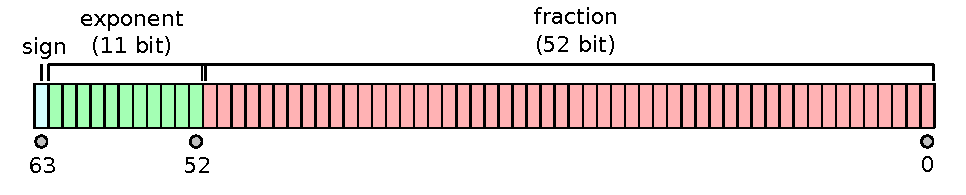
\includegraphics[width=1\textwidth]{pdf/double.pdf}
    \caption{Bitová reprezentace čísla v plovoucí řádce s dvojitou přesností dle IEE 754}
\end{figure}

Při ponechání prvních 12 bitů rozdělujeme interval čísel v plovoucí čárce na $2^{12}$ podintervalů.
Samotný výpočet podintervalu, do kterého zpracovávané číslo patří, je tedy realizovaný pomocí bitového posunu o 52 bitů doprava.

Dalším důsledkem bitové reprezentace čísel typu \texttt{double} je to, že pokud budeme ponechávat více než prvních 12 bitů (tedy když budeme ponechávat i bity mantisy), porovnávání dvou takových čísel zústane stále stejné.
Pomocí počtu bitů, které budeme posouvat, lze tedy jednoduše tedy konfigurovat počet podintervalů.

V případě, že by se v nějakém podintervalu i tak vyskytovalo příliš mnoho unikátních čísel, a nebylo by možné ho dále zpracovávat, je možné ponechávat dalších $n$ bitů následujících po bitech, které jsme ponechali při původním sestrojování histogramu, čímž podinterval rozdělíme na další podintervaly.

Rozdělování čísel do podintervalů pomocí bitového posunu poskytuje rychlý a jednoduchý způsob, jak rozdělovat čísla typu \texttt{double} do podintervalů, a tak efektivně sestavovat histogram i pro soubory, které se nevejdou do operační paměti.

\subsection{Paralelizace vyhledání percentilu}
Jelikož postup pro vyhledání percentilu v souboru uvedený v sekci \ref{bucketing} je velmi jednoduchý a výpočetně nenáročný, tak se zdá, že hlavním faktorem, který bude ovlivňovat dobu vyhledávání, bude rychlost čtení ze souboru (tedy přístup k IO).
Důsledkem toho je tedy efektivní paralelizace tohoto výpočtu složitá, jelikož čas strávený čekáním na IO je násobně větší než čas strávený sestavováním histogramu a jeho zpracováním za účelem vyhledání percentilu.

Jedním ze způsobů, jak provést paralelní vyhledávání percentilu, je takový způsob, kdy jedno vlákno čte ze souboru, a pomocí kruhového bufferu předává načtená data (čísla) dalším vláknům, která je zpracovávají. Výsledky výpočtů pak ukládají pomocí řízeného přístupu do chráněné paměti histogramu tak, aby nedošlo ke konfliktům. 
Další variantou tohoto způsobu, když zvolíme správnou velikost podintervalů, je způsob, kdy si každé vlákno sestavuje svůj vlastní histogram, a po přečtení celého souboru jsou histogramy vláken zkombinovány do jednoho hlavním vláknem, přičemž tato varianta je náročnější na velikost používaného paměťového prostoru výměnou za teoreticky rychlejší dobu vyhledávání z důvodu nepřítomnosti synchronizace při přístupú do sdílené paměti histogramu.

\begin{figure}[!ht]
    \centering 
    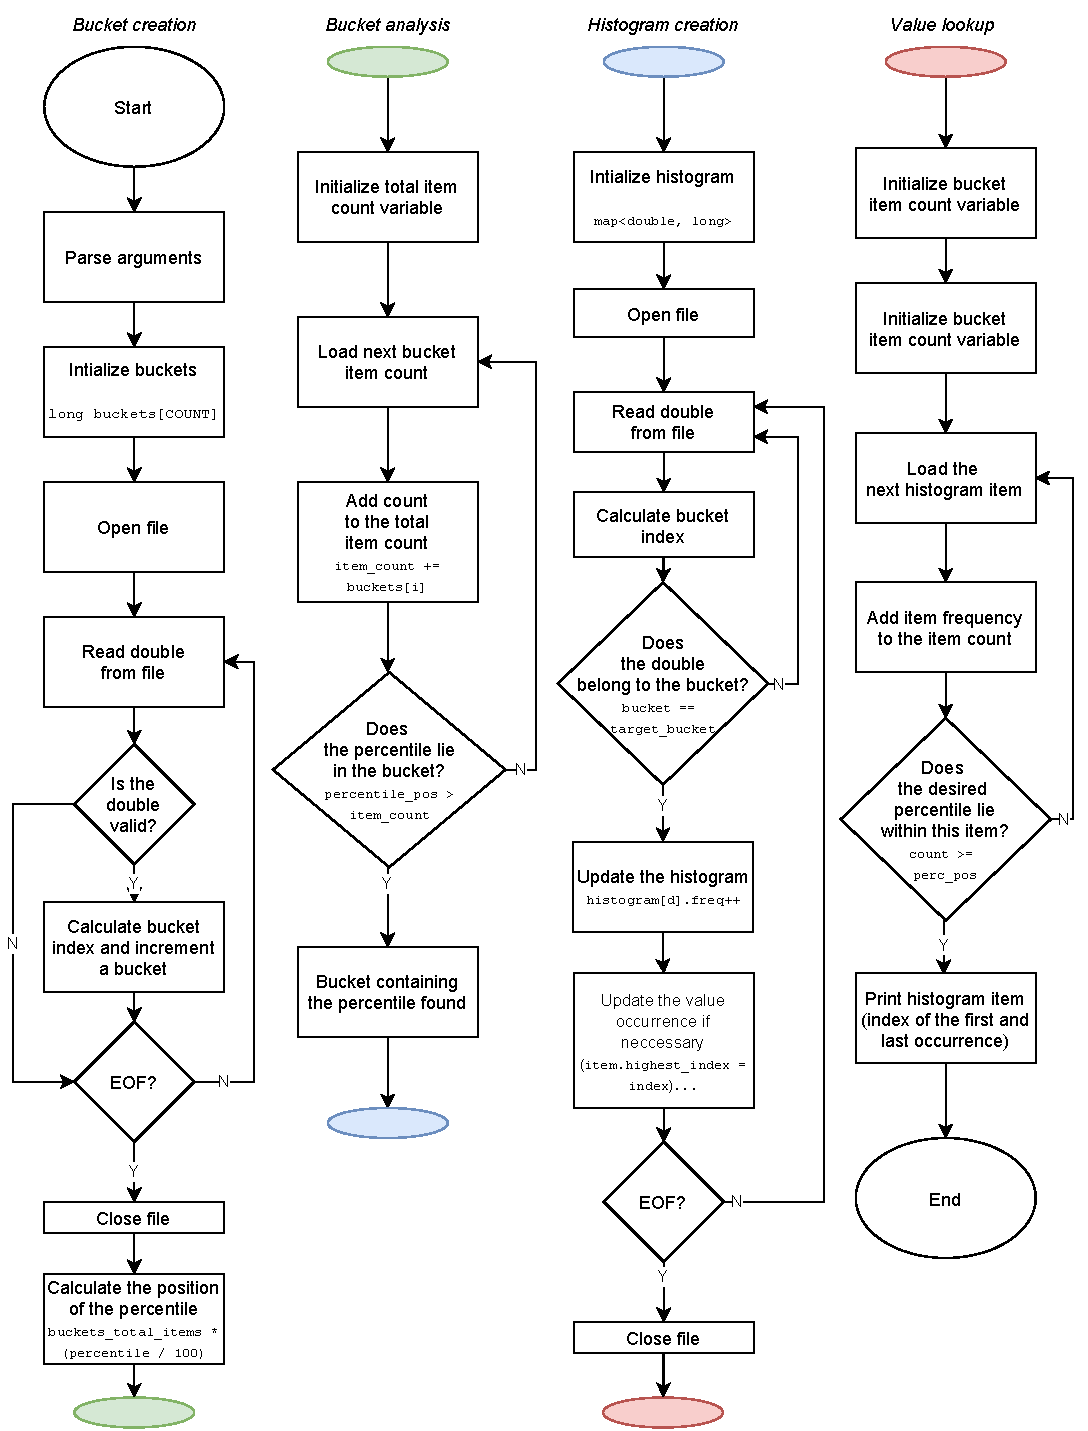
\includegraphics[width=1.038125\textwidth]{pdf/cfd.pdf}
    \caption{Diagram typu control-flow znázorňující zjednodušený postup používaný při vyhledávání percentilu v souboru s omezenou operační pamětí}
\end{figure}


\section{Popis implementace}

K vyhledávání percentilů v souborech byl zvolen postup popsaný v sekci \ref{bucketing} nakonfigurovaný tak, aby bylo během sestavování histogramu ponecháváno prvních \bucketingparamone~bitů čísla.
Pokud by se v podintervalu, ve kterém se nachází percentil, nacházelo příliš mnoho unikátních čísel, tak by se znovu spustilo sestavování histogramu, aby se počet unikátních čísel redukoval. 
Podinterval, ve kterém se nachází percentil, by se dělil na další podintervaly tak, že by se po původních \bucketingparamone~bitech ponechávalo i dalších \bucketingparamtwo~bitů. 
V každém podintervalu by tak mohlo být maximálně $2^{\bucketingparamthree}$~unikátních čísel.

\subsection{Sériová implementace}
Sériová implementace, při které probíhá výpočet jen na jednom vlákně, je velmi jednoduchá, a nachází se ve zdrojovém souboru \texttt{serial\_bucketing.cpp}.

%, kde jsou definovány dvě hlavní funkce: \texttt{create\_buckets\_serial} a \texttt{create\_buckets\_serial}.

Funkce \texttt{create\_buckets_serial} sestavuje histogram z čísel nacházejících se ve vstupním souboru.
Velikost histogramu je daná počtem bitů, které jsou z každého načteného čísla ponechávány.

Po sestavení histogramu se vypočítá podinterval, ve kterém se percentil nachází, a přesná pozice relativní vůči seřazeným číslům nacházejících se v souboru. 

Poté se ve funkci \texttt{find\_percentile\_value\_serial} znovu čte celý vstupní soubor, ale zpracovávají se pouze čísla, která patří do výsledného podintervalu.
Výskyt každého zpracovávaného čísla je zaznamenáván do dalšího histogramu (již implementován pomocí datové struktury tabulka). 
Dále se také pro každé číslo zaznamenává jeho první a poslední výskyt v souboru.

Nakonec, po zpracování celého souboru, je z histogramu, dle předtím vypočítané pozice, vybráno konkrétní číslo (včetně jeho výskytů), které je považováno za hledaný percentil.

Díky výpočtu percentilu pomocí bitového posunu a následné aktualizaci histogramu pomocí $O(1)$ operace (zápis dle indexu do \texttt{std::vector}) je sériová implementace velmi rychlá.

\section{Závěr}

\end{document}

